\documentclass[]{article}
\usepackage{lmodern}
\usepackage{amssymb,amsmath}
\usepackage{ifxetex,ifluatex}
\usepackage{fixltx2e} % provides \textsubscript
\ifnum 0\ifxetex 1\fi\ifluatex 1\fi=0 % if pdftex
  \usepackage[T1]{fontenc}
  \usepackage[utf8]{inputenc}
\else % if luatex or xelatex
  \ifxetex
    \usepackage{mathspec}
  \else
    \usepackage{fontspec}
  \fi
  \defaultfontfeatures{Ligatures=TeX,Scale=MatchLowercase}
\fi
% use upquote if available, for straight quotes in verbatim environments
\IfFileExists{upquote.sty}{\usepackage{upquote}}{}
% use microtype if available
\IfFileExists{microtype.sty}{%
\usepackage{microtype}
\UseMicrotypeSet[protrusion]{basicmath} % disable protrusion for tt fonts
}{}
\usepackage[unicode=true]{hyperref}
\hypersetup{
            pdfborder={0 0 0},
            breaklinks=true}
\urlstyle{same}  % don't use monospace font for urls
\usepackage{graphicx,grffile}
\makeatletter
\def\maxwidth{\ifdim\Gin@nat@width>\linewidth\linewidth\else\Gin@nat@width\fi}
\def\maxheight{\ifdim\Gin@nat@height>\textheight\textheight\else\Gin@nat@height\fi}
\makeatother
% Scale images if necessary, so that they will not overflow the page
% margins by default, and it is still possible to overwrite the defaults
% using explicit options in \includegraphics[width, height, ...]{}
\setkeys{Gin}{width=\maxwidth,height=\maxheight,keepaspectratio}
\IfFileExists{parskip.sty}{%
\usepackage{parskip}
}{% else
\setlength{\parindent}{0pt}
\setlength{\parskip}{6pt plus 2pt minus 1pt}
}
\setlength{\emergencystretch}{3em}  % prevent overfull lines
\providecommand{\tightlist}{%
  \setlength{\itemsep}{0pt}\setlength{\parskip}{0pt}}
\setcounter{secnumdepth}{0}
% Redefines (sub)paragraphs to behave more like sections
\ifx\paragraph\undefined\else
\let\oldparagraph\paragraph
\renewcommand{\paragraph}[1]{\oldparagraph{#1}\mbox{}}
\fi
\ifx\subparagraph\undefined\else
\let\oldsubparagraph\subparagraph
\renewcommand{\subparagraph}[1]{\oldsubparagraph{#1}\mbox{}}
\fi

% set default figure placement to htbp
\makeatletter
\def\fps@figure{htbp}
\makeatother


\date{}

\begin{document}

Lezione 30-11-2016

Argomento: SSN, prevenzione e screening

Docente: professor Signorelli

Sbobinatore: Marina Agrusta

Sezione: Politiche di prevenzione

Prestazioni erogate dal SSN gratuitamente o con compartecipazione di
spesa (ticket) :

\begin{itemize}
\item
  Medico di famiglia
\item
  Pronto Soccorso
\item
  Ricoveri ospedalieri acuti o lungodegenti
\item
  Prestazioni specialistiche ambulatoriali
\item
  Esami diagnostici e di laboratorio
\item
  Farmaci per malattie rilevanti (classe A)
\item
  Vaccinazioni
\item
  Screening oncologici
\end{itemize}

Ci concentreremo principalmente su questi due ultimi punti in tema di
prevenzione. Un istituto privato che ha stimato il Fondo Sanitario ha
documentato che rispetto ai 113 miliardi di euro che sono previsti, ci
sarebbero dei risparmi su : 7 miliardi di sovra-utilizzo di strutture, 5
miliardi di frodi e abusi, 3 miliardi di acquisti a costi eccessivi, 3.4
miliardi di sotto-utilizzo di posti letto vuoti, complessità
amministrative (quello che riusciamo a gestire meno), 3 miliardi per
l'inadeguato coordinamento dell'assistenza. Si preme soprattutto per
migliorare gli ultimi due punti.

QUIZ

Rientrano tra le prestazioni attualmente erogate gratuitamente dal SSN a
tutti i cittadini:

\begin{enumerate}
\def\labelenumi{\arabic{enumi}.}
\item
  Medico di famiglia
\item
  Pediatra di libera scelta
\item
  Ricoveri ospedalieri
\item
  Day hospital
\end{enumerate}

\begin{enumerate}
\def\labelenumi{\alph{enumi})}
\item
  1
\item
  1,2
\item
  1,2,3,4
\item
  1,3,4
\item
  1,2,3
\end{enumerate}

Ovviamente la risposta è la c, perché se ci fossero state le cure
omeopatiche, odontoiatriche e estetiche allora potevamo avere dei dubbi

Il problema più rilevante della sanità pubblica italiana è attualmente:

\begin{enumerate}
\def\labelenumi{\alph{enumi})}
\item
  Epidemie di malattie infettive
\item
  Numero di morti per AIDS
\item
  Sostenibilità economica del sistema sanitario
\item
  Eccessivo numero di medici
\item
  Carenza di personale medico
\end{enumerate}

La risposta è la c.

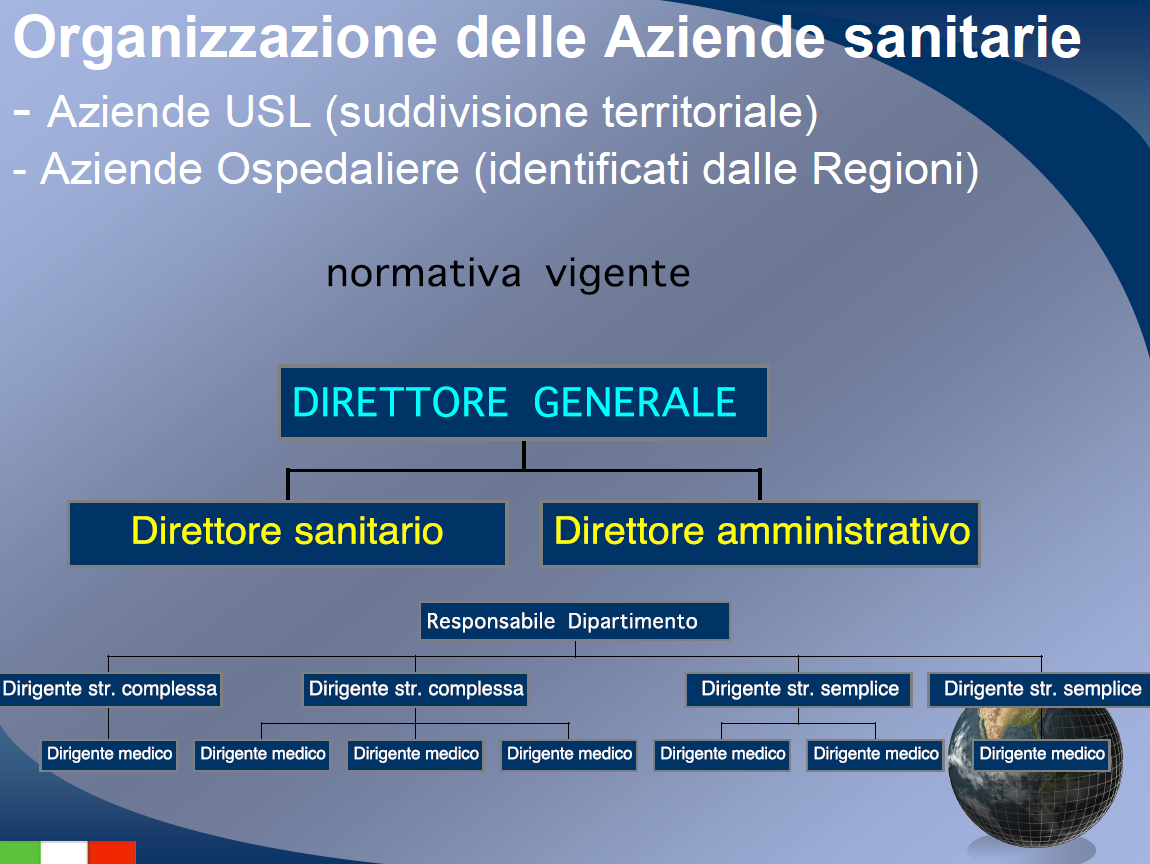
\includegraphics[width=6.69306in,height=4.72639in]{media/image1.png}

Notizia apparsa oggi sui giornali specializzati in tema di salute:
tassare il fumo, il cibo spazzatura, le bevande gassate e la guida
pericolosa. Tra il dirlo e il farlo passa molto anche perchè non puoi
dire a qualcuno ``non ti curo perchè fumi'' anche perchè sappiamo che il
fumo contribuisce ma non è il determinante principale. Questi concetti
comunque rientrano in un concetto generale detto Health in all policies,
diverso dall'one health visto nei determinanti di salute, stiamo
parlando di una precisa politica dell'UE che dice che per garantire il
miglior stato di salute occorre che tutte le leggi e i provvedimenti in
vari ambiti, considerino la ricaduta sulla salute. Ad esempio fa
riferimento a fiscalità, ricerca, ambiente, politica sociale regionale e
istruzione. Quindi ci occupiamo anche di come regolare le tassazioni,
per esempio ci sono delle politiche che dicono ``chi inquina di più
paga'' (esempio di Milano e sulla tassazione delle macchine in centro
basata su quanto inquina la macchina).

Quindi i decisori politici devono essere sensibilizzati per le ricadute
sulla salute e il benessere delle persone.

Sottosottosezione: \textbf{Classificazione della prevenzione}

\begin{itemize}
\item
  prevenzione primaria: rimuovere i fattori di rischio e proteggere gli
  esposti (es. vaccini)
\end{itemize}

\begin{itemize}
\item
  prevenzione secondaria: diagnosi precoce e identificazione di
  situazioni a rischio
\item
  prevenzione terziaria: riabilitazione malati cronici e prevenzione
  delle complicanze
\end{itemize}

Altra classificazione:

\begin{itemize}
\item
  prevenzione attiva: sul singolo (vaccini, screening) e include sia la
  primaria che la secondaria
\item
  prevenzione collettiva
\end{itemize}

Sottosottosezione: \textbf{Medicina Predittiva} (introdotta nel piano
nazionale di prevenzione 2010-12)

La medicina predittiva è una forma di medicina preventiva che ha lo
scopo di definire dei protocolli di prevenzione individuali. Es il
predisposto al diabete deve controllare la sua glicemia tutti gli anni.
La speranza in futuro è individuare le predisposizioni genetiche grazie
all'ingegneria genetica, così da poter fare una reale prevenzione
primaria. È rivolta agli individui sani, cerca fragilità o difetti che
predispongono alla malattia, consente la personalizzazione di interventi
creando profili di rischio e monitoraggi (es. mappature genetiche, carta
del rischio). Il concetto è ottimizzare gli interventi.

Sottosottosezione: \textbf{Malattie croniche: un allarme mondiale}

\begin{itemize}
\item
  57 milioni di decessi nel 2008
\item
  il 63\% (36 milioni) dovuto a malattie croniche non trasmissibili
\item
  25\% circa di morti sotto i 60 anni (morte prevedibili)
\item
  primo posto: malattie cardiovascolari(48\%) seguite dai tumori(21\%),
  malattie respiratorie croniche(12\%) e diabete( 3,5\% ma sempre più in
  aumento).
\end{itemize}

Ovviamente stiamo facendo riferimento ai paesi industrializzati.

In Italia : malattie cardiovascolari (41\% delle morti), tumori(30\%)
con incidenza in aumento ogni anni(250.000 nuovi casi/anno), terza causa
malattie respiratorie croniche, ultimo diabete con 3,000,000 malati( 5\%
della popolazione) e 1 milione di diabetici che non sanno di esserlo, e
questo è un grosso problema perchè non controllano la loro glicemia
nelle prime fasi quindi aumentano le complicanze.

Paragrafo: \textbf{Strategia italiana}

\begin{itemize}
\item
  conoscere e monitorare i fenomeni (sorveglianze)
\item
  promuovere stili di vita salutari a partire dai primi anni di vita e
  ancora prima ( in gravidanza)
\item
  prevenzione ambientale con ambienti più salutari di vita e di lavoro (
  a partire dalla scuola)
\item
  facilitare comportamenti e scelte salutari
\item
  empowerment (cittadino)
\item
  coerenza di sistema (decisore politico): one healt e healt in all
  policies
\end{itemize}

Il ministero ha un Piano Sanitario Nazionale e un Piano Nazionale della
Prevenzione i quali obiettivi sono: alimentazione, attività fisica,
alcol (le modiche quantità non creano problemi) e fumo (ci sono da
aggiungere anche le droghe).

Sottosottosezione: \textbf{problemi delle iniziative di prevenzione in
Italia}

\begin{itemize}
\item
  scarsa cultura scientifica in riferimento standard internazionali
\item
  interessi confliggenti e crisi economica (esempio di Taranto e
  dell'Ilva, e del conflitto tra inquinamento e posti di lavoro. Se oggi
  ci dicessero ``dal punto di vista ambientale abbiamo risolto tutto e
  si può continuare a lavorare'' come potremmo sapere che effettivamente
  è vero? Le morti di oggi sono sicuramente dovute all'inquinamento di
  qualche anno fa, quindi i problemi eventuali li vedremmo sul lungo
  termine)
\item
  bilanci di governo organizzati in ``silos'' dove ognuno pensa al suo
  ambito quando invece dovrebbe esserci una piena collaborazione
\item
  investimenti vs entrate tributarie: paradosso tra le campagne antifumo
  promosse dallo stato e le accise guadagnate sul commercio del tabacco.
  Se tutti seguissimo i consigli dello stato allora andrebbe in rovina
  il sistema tributario.
\item
  Resistenza dei gruppi antagonisti (es antivaccini, chi rifiuta le
  analisi o cure oppure chi ne vuole troppe\ldots{}vedi il caso Stamina)
\item
  Scarsa visibilità della sanità pubblica e della prevenzione rispetto
  alla clinica e la riabilitazione
\item
  La prevenzione costa, anche se poco
\item
  Impatto e rendita economico-finanziaria su tempi lunghi con evidenze
  di tipo probabilistico
\end{itemize}

Sottosottosezione: \textbf{Le pipeline nazionali}

\begin{itemize}
\item
  Piano screening oncologici
\item
  Piano nazionale della fertilità
\item
  Piano nazionale delle demenze
\item
  Piano nazionale per la prevenzione delle epatiti B e C
\item
  Piano nazionale amianto (mai effettuato perché manca la copertura
  economica)
\item
  Piano nazionale vaccini
\item
  Piano nazionale genomica e epigenetica
\end{itemize}

sottosottoSezione: \textbf{Piano Nazionale della prevenzione 2014-2018}

Identifica dieci macro obiettivi :

\begin{enumerate}
\def\labelenumi{\arabic{enumi}.}
\item
  Ridurre il carico di morbosità, mortalità e disabilità delle malattie
  non trasmissibili
\item
  Prevenire le conseguenze dei disturbi neurosensoriali
\item
  Promuovere il benessere mentale nei bambini, adolescenti e giovani
\item
  Prevenire le dipendenze da sostanze
\item
  Prevenire gli incidenti stradali o ridurre la loro gravità
\item
  Prevenire gli incidenti domestici
\item
  Prevenire gli infortuni e le malattie professionali
\item
  Ridurre le esposizioni ambientali potenzialmente dannose per la salute
\item
  Ridurre la frequenza di infezioni
\item
  Attività di prevenzione in sicurezza alimentare e veterinaria
\end{enumerate}

La prevenzione delle malattie è un tema molto sentito dalle popolazioni
e quindi potenziale fonte di consenso politico. Il politico abile può
creare consenso anche in tempi brevi proponendo interventi di
prevenzione con messaggi chiari e efficaci. Ciò è indipendente dalla
reale efficacia dell'intervento che può anche risentirne negativamente.

Compito degli esperti di sanità pubblica è quello di influenzare i
decisori sulle più recenti evidenze scientifiche ma anche
sull'importanza delle iniziative di prevenzione come mezzo per lo
sviluppo sociale ed economico di un paese e cercando di fermare con
argomenti scientifici le strumentalizzazioni e le derive demagogiche
(esempio sempre metodo stamina e di come i politici stessi sono in
difficoltà per le richieste della popolazione. Per questo ci sono gli
esperti).

Paragrafo: \textbf{Spesa in prevenzione in Italia}

Quanto spendiamo per la prevenzione in Italia? Il 4,2\% della spesa
sanitaria. Abbiamo presentato uno studio qualche settimana fa su
regioni, tipo la Calabria, che spendono di più per la prevenzione in
realtà lo fanno per il costo del personale, non perchè siano virtuose.
Quindi in realtà di prevenzione se ne fa poca e la spesa così alta è
spiegata in altro modo.

Carrellata sulle coperture vaccinali: abbiamo un divario tra le diverse
regioni, soprattutto per le informazioni riportate. Ci sono regioni che
non hanno un'anagrafe vaccinale (e non si parla solo di regioni del sud
Italia), quindi non è possibile avere dati attendibili. Paradossalmente
è più dettagliato il registro vaccinale dei bovini che quello della
popolazione.

Per quanto riguarda la copertura per il morbillo, nel 2014 è andata
male, per il 2015 meglio, il problema è far capire alle persone il
concetto di immunità di gregge, perchè in questo modo riusciamo a
proteggere chi effettivamente non può vaccinarsi, un po' come l'epidemia
avvenuta a Disneyland qualche anno fa dove i primi responsabili furono i
dipendenti e la popolazione americana, che non essendo vaccinati
infettarono anche persone che venivano da paesi dove la copertura
vaccinale non era garantita al meglio.

Parlando della rosolia congenita abbiamo riscontrato in Italia 78 casi
di rosolia congenita negli ultimi 10 anni, e soprattutto in Campania,
non perchè ci siano degli oppositori, ma perchè non è organizzato il
programma vaccinale.

Questo è l'andamento del vaccino anti influenzale, quest'anno
sicuramente avremo una risposta maggiore.

(parla in riferimento ai grafici delle slides dell'obesità in Italia,
sempre evidenziando la diversità tra le regioni e come anche le malattie
future seguiranno questo andamento)

Sottosottosezione: \textbf{Alcune definizioni}

\begin{itemize}
\item
  \textbf{Empowerment}: è il processo attraverso il quale le persone
  acquisiscono un maggiore controllo rispetto alle decisioni e alle
  azioni che riguardano la propria salute. Può essere un processo
  sociale, culturale, psicologico o politico attraverso il quale gli
  individui e i gruppi sociali sono in grado di esprimere i propri
  bisogni e le proprie preoccupazioni, individuare le strategie per
  essere coinvolti nel processo decisionale e intraprendere azioni di
  carattere politico, sociale culturale che consentono loro di
  soddisfare tali bisogni.
\item
  \textbf{Counselling}: nell'ambito sanitario, è un'attività
  relazionale, svolta da personale specializzato, finalizzata a
  orientare, sostenere e sviluppare le potenzialità di persone
  momentaneamente in difficoltà.
\item
  \textbf{Advocacy}: combinazione di azioni individuali e sociali volte
  ad ottenere impegno politico, sostegno alle politiche, consenso
  sociale e sostegno dei sistemi sociali per un particolare obiettivo o
  programma di salute. Questo tipo di azione dovrebbe essere intrapresa
  da e/o per conto di individui o gruppi, al fine di creare condizioni
  di vita favorevoli alla salute e di ottenere stili di vita salutari.
\item
  \textbf{Healt literacy}: l'alfabetizzazione alla salute comprende le
  abilità cognitive e sociali che determinano la motivazione e la
  capacità degli individui di accedere alle informazioni, di
  comprenderle e utilizzarle in modo da promuovere e mantenere una buona
  salute.
\end{itemize}

Sottosezione: \textbf{Screening}

Definizione Who: processo attraverso il quale le malattie non
riconosciute (o difetti) sono identificate attraverso test che possono
essere applicati rapidamente e su larga scala. Prende le persone
apparentemente sane tra quelle a rischio.

I programmi di screening dovranno prevedere: la predisposizione di linee
guida per la conferma diagnostica dei casi sospetti identificati ed il
trattamento tempestivo dei casi confermati, l'istituzione di un sistema
di controllo di qualità dei programmi di diagnosi precoce.

{[}Excursus sul Psa: alla fine Signorelli afferma che è un test poco
sensibile, perchè è utile per chi ha i sintomi e non per chi è
asintomatico perchè i falsi positivi sono troppi. Quindi è inserito tra
gli screening di dubbia efficacia.{]}

\textbf{ELENCO SCREENING UTILIZZATI IN ITALIA}

SCREENING DI MASSA IN POPOLAZIONI ADULTE

\begin{itemize}
\item
  tumore della cervice uterina: pap-test
\item
  tumore della mammella: mammografia
\item
  tumore del colon-retto: ricerca del sangue occulto nelle feci
\end{itemize}

SCREENING SELETTIVI IN SOGGETTI CON FAMILIARITà

\begin{itemize}
\item
  Diabete mellito: glicemia
\item
  glaucoma: pressione intraoculare
\item
  ipertensione: pressione
\item
  malattie cardiovascolari: vari esami strumentali
\item
  tumore colon-retto con poliposi familiare: colonscopia
\end{itemize}

SCREENING DI DUBBIA EFFICACIA

\begin{itemize}
\item
  tumore alla prostata: psa
\item
  tumori cutanei
\item
  tumori dei brochi: esame dell'espettorato
\item
  tumore del polmone: rx torace
\item
  seminomi testicolari: palpazione
\item
  ulcera gastrica e duodenale: IgG per H. Pylori
\item
  tumore dello stomaco: gastroscopia
\end{itemize}

SCREENING DI MASSA IN Età NEONATALE

funzionano tutti: displasia congenita dell'anca, ipotiroidismo congenito
ecc...

SCREENING PER LA TUTELA DELLA POPOLAZIONE SANA

Di solito malattie infettiva: HIV,HBV,HCV, malattie a trasmissione
fecale-orale...

SCREENING PRECONCEZIONALI E PRENATALI

Malattie genetiche

SCREENING IN AMBITO LAVORATIVO E SPORTIVO

Sordità, funzionalità respiratoria, patologie cardiache latenti,
alterazioni oculari ecc...

Importanti in concetti di Sensibilità e Specificità soprattutto ai fini
dell'esame.

Sensibilità: probabilità del test positivo nelle persone con malattia

Specificità: probabilità del test negativo nelle persone senza malattia.
Meglio prendere qualche falso positivo che farsi sfuggire un falso
negativo. E questo lo valuto soprattutto al momento della soglia da
scegliere per definire i falsi positivi e i falsi negativi.

\end{document}
